\documentclass[10pt,conference]{IEEEtran}

% ============================================================
% Packages
% ============================================================
\usepackage[T1]{fontenc}
\usepackage[utf8]{inputenc}
\usepackage{times}
\usepackage{microtype}
\usepackage{graphicx}
\usepackage{booktabs}
\usepackage{array}
\usepackage{tabularx}
\usepackage{enumitem}
\usepackage{xcolor}
\usepackage{hyperref}
\usepackage{minted}
\usepackage{amsmath}
\usepackage{amssymb}

\hypersetup{
    colorlinks=true,
    linkcolor=blue,
    citecolor=blue,
    urlcolor=blue
}

\setlist[itemize]{leftmargin=*, itemsep=2pt, topsep=2pt}
\setlist[enumerate]{leftmargin=*, itemsep=2pt, topsep=2pt}
\setminted{fontsize=\footnotesize,breaklines=true,frame=single,autogobble=true}

% ============================================================

% ============================================================
% Title
% ============================================================
\title{
Assignment 2 Report Template:\\
Domain Adaptation with Small Language Models
}

\author{
\IEEEauthorblockN{
Group Number: \emph{Insert Group Number}
}
\IEEEauthorblockA{
CSCI433/933 Machine Learning Algorithms and Applications\\
Student Names and Student Numbers: \emph{Insert Details}\\
}
}

\usepackage{tikz}
\usetikzlibrary{shapes.geometric, arrows.meta, positioning}

\begin{document}
\maketitle

% ============================================================
\section{Methodology}
\label{sec:methodology}

This project adapts Gemma~3~4B, a pretrained small language model 
running locally via Ollama, for Shakespeare question answering using 
retrieval-augmented generation (RAG) as the primary adaptation strategy. 
Rather than modifying the model's weights, the system conditions the 
model's responses on passages retrieved directly from the Shakespeare 
corpus at query time. Three systems were implemented and compared: a 
prompt-only baseline that relies solely on the model's pretrained 
knowledge, a standard RAG system that retrieves relevant utterances 
from an indexed corpus before generating an answer, and an enhanced 
RAG system that extends retrieval with cross-encoder reranking and 
scene-level diversity filtering. All three systems use the same language 
model and hardware setup, isolating retrieval and reranking as the 
variables under evaluation.

\subsection{Baseline System}

The baseline system is implemented in \texttt{baseline.py} and performs no retrieval. A user
question is formatted using a prompt template and sent directly to Gemma~3~4B via Ollama.
The model generates its answer solely from its pretrained weights, with access only to the
user's question and its general training knowledge --- it has no access to the Shakespeare
corpus, retrieved passages, or any scene metadata at query time.

This is a prompt-only baseline rather than a scene-level retrieval baseline. This choice was
deliberate: a no-retrieval baseline produces a cleaner separation between the two systems,
making the contribution of retrieval directly measurable. When the model lacks retrieved
context, failures such as hallucination, vague answers, and unsupported claims become visible
and attributable to the absence of retrieval rather than to poor retrieval quality.

The baseline uses the same language model, hardware, and prompt structure as the improved
system. This ensures that any difference in output quality between the two systems is
attributable to the presence or absence of retrieval, not to differences in model capability
or infrastructure.

\subsection{RAG-Based System}

\subsubsection{Standard RAG-Based System}

The improved system retrieves from the \texttt{shakespeare\_utterances} ChromaDB collection,
built by the data engineering pipeline. Each utterance was indexed using an enriched
embedding string combining the speaker, utterance text, scene summary, and keywords ---
providing the embedding model sufficient semantic context to represent short archaic lines
meaningfully in vector space. The RAG pipeline queries this pre-built index directly at
runtime, with no recomputation required.

At query time, the user's question is embedded using
\texttt{sentence-transformers/all-MiniLM-L6-v2}, which maps any text string into a
384-dimensional vector space. This vector is compared against the indexed utterance vectors
via ChromaDB's approximate nearest-neighbour index. Because the embedding model was trained on large modern English
corpora, it understands semantic proximity between contemporary
query language and archaic Shakespearean phrasing --- meaning a
query such as ``Why does Macbeth kill Duncan?'' can surface relevant
passages even when the exact words ``kill'' or ``Duncan'' do not
appear in them. This works because words such as ``kill'',
``murder'', and ``do the deed'' occupy nearby regions of vector
space regardless of surface form. The enriched embedding strings
--- which include modern English scene summaries and keywords
alongside the archaic utterance text --- further bridge the
vocabulary gap, ensuring that short Shakespearean lines are placed
in semantically meaningful positions rather than isolated by their
archaic phrasing.
The top-$k$ results are returned with full
metadata including play, act, scene, speaker, and scene summary. Retrieved passages are
always displayed to the user before the generated answer, regardless of interaction mode.
This guarantees transparency --- the user can always see what context the model was given
before reading its response.

The system supports four interaction modes. In \texttt{qa} and \texttt{concept} modes,
retrieved utterances are formatted into a structured context block --- including provenance
labels and scene context --- and injected into a prompt template alongside the user's
question. In \texttt{evidence} mode, generation is skipped entirely and only the retrieved
passages are displayed. In \texttt{stylised} mode, a separate prompt template requests a
Shakespearean-style response limited to 150 words, and the output is explicitly labelled as
creative rather than factual, clearly distinguishing it from evidence-based answers. Prompt
templates are stored as external files, decoupling prompt design from pipeline logic and
allowing iterative refinement without code changes.

\subsubsection{Enhanced RAG-Based System}

An enhanced pipeline extends the standard system with a two-stage retrieve-then-rerank
approach. In the first stage, ChromaDB retrieves 15 broad candidates using the bi-encoder,
where query and document vectors are computed independently and compared by cosine
similarity. While fast, this approach can miss fine-grained relevance because the query and
document are never directly compared against each other. In the second stage, a cross-encoder
model (\texttt{cross-encoder/ms-marco-MiniLM-L-6-v2}) addresses this by jointly processing
each query--document pair as a single input, allowing the model to attend to the interaction
between query terms and document terms directly. This produces more accurate relevance scores
at the cost of higher computation, which is why the cross-encoder is applied only to the
shortlisted 15 candidates rather than the full collection. Candidates are then re-sorted by
cross-encoder score before the top-5 are selected for generation.

A scene-level diversity constraint of at most two results per scene is applied after
reranking. This prevents a single highly relevant scene from dominating the context block,
which is particularly important for multi-act questions such as Q3 (Hamlet's delay), where
evidence spans several separate scenes across the play. That said, this constraint is a
known limitation: for focused single-scene questions, it may discard highly relevant
passages in favour of less relevant ones from other scenes. A minimum coverage constraint
--- guaranteeing at least one result per act rather than capping per scene --- may be a
more appropriate strategy and is identified as a direction for improvement.

\subsection{Model Choice and Justification}
 
Gemma~3~4B was selected as the language model for both the baseline and improved systems,
running locally via Ollama. Table~\ref{tab:model_comparison} summarises the five candidate
models evaluated before this decision was made.
 
\begin{table}[ht]
\centering
\caption{Candidate model comparison. RAM figures sourced from official
Ollama model pages~\cite{ollama_gemma3,localaimaster_ram}.
RAG evaluation score reflects whether the model's limited domain
knowledge makes retrieval genuinely necessary.}
\label{tab:model_comparison}
\begin{tabular}{llcc}
\hline
\textbf{Model} & \textbf{Type} & \textbf{RAM} & \textbf{RAG eval genuine} \\
\hline
\textbf{Gemma 3 4B}  & Local & $\sim$2.5\,GB~\checkmark & 5/5 \\
Mistral 7B Q4        & Local & $\sim$4.3\,GB~$\approx$  & 5/5 \\
Gemma 4 E4B          & Local & $\sim$8\,GB~$\times$     & 5/5 \\
Phi-4 Mini           & Local & $\sim$2.3\,GB~\checkmark & 5/5 \\
TinyLlama 1.1B       & Local & $\sim$0.7\,GB~\checkmark & 5/5 \\
Gemini Flash         & API   & 0\,GB (hosted)           & 1/5 \\
\hline
\end{tabular}
\end{table}
 
The deciding hardware constraint was the group's weakest machine at 8\,GB RAM. At
approximately 2.5\,GB under 4-bit quantisation~\cite{google_gemma3_qat}, Gemma~3~4B runs
comfortably on every group member's laptop without requiring specialised hardware or GPU
resources. Mistral 7B Q4 was eliminated despite comparable quality because its
4.3\,GB footprint leaves insufficient headroom on 8\,GB systems once the OS and other
applications consume memory~\cite{mistral_vram}. Gemma~4 E4B was eliminated entirely as its
memory requirement sits at the 8\,GB ceiling~\cite{google_gemma4}. Phi-4 Mini fits the RAM
constraint but is optimised for reasoning and STEM tasks~\cite{phi4_mini_benchmark}, making
it a poor fit for the stylised generation mode. TinyLlama 1.1B, while the smallest option,
has been shown to struggle with nuanced synthesis tasks~\cite{tinyllama_eval}, which this
assignment requires.
 
The choice of a local model over a hosted API was deliberate. Gemma~3~4B has limited
knowledge of Shakespearean text, meaning that retrieval quality directly and visibly impacts
answer quality. When relevant passages are retrieved, the model produces accurate, grounded
answers. When retrieval fails, the model's response degrades noticeably. This makes the
comparison between the baseline and RAG system meaningful and the evaluation genuine. A
powerful hosted model such as Gemini Flash already has strong Shakespeare knowledge and may
produce correct answers even without retrieved context, which would make evaluation
inconclusive and undermine the purpose of the RAG pipeline.
 
Gemma~3~4B also demonstrates reliable instruction following and sufficient language quality
for both beginner-friendly explanation and stylised generation, making it appropriate for all
four interaction modes the system supports.

% ============================================================
\section{System Design and Implementation}
\label{sec:system}

% ---------------------------------------------------------------
% RAG System Pipeline Diagram — Three Balanced Columns
% Requires in preamble:
%   \usepackage{tikz}
%   \usetikzlibrary{arrows.meta}
% ---------------------------------------------------------------

\begin{figure*}[ht]
\centering
\scalebox{0.78}{
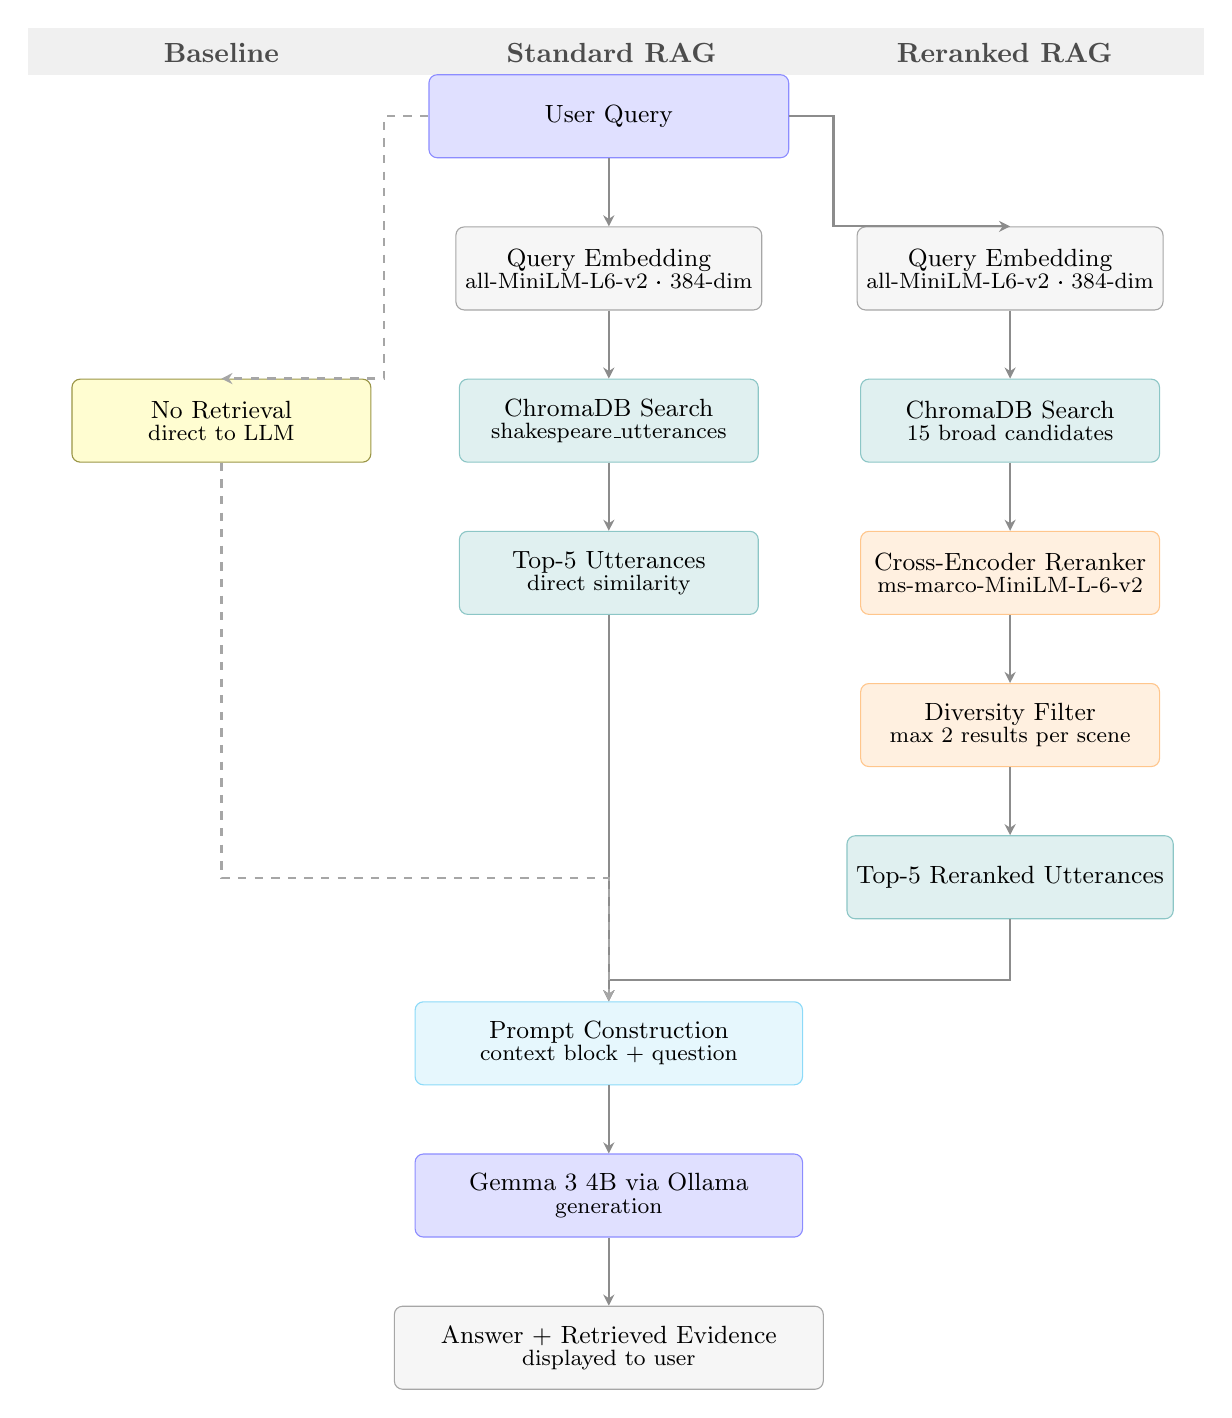
\begin{tikzpicture}[x=1pt, y=1pt]

\tikzset{
  box/.style      = {rectangle, rounded corners=3pt, minimum width=108pt,
                     minimum height=30pt, align=center, font=\small,
                     draw=black!35, fill=gray!7, text=black},
  purple/.style   = {box, fill=blue!12,   draw=blue!45},
  teal/.style     = {box, fill=teal!12,   draw=teal!45},
  coral/.style    = {box, fill=orange!12, draw=orange!45},
  blue/.style     = {box, fill=cyan!10,   draw=cyan!45},
  amber/.style    = {box, fill=yellow!18, draw=yellow!55!black},
  arr/.style      = {-{Stealth[length=4pt,width=4pt]}, thick, black!45},
  darr/.style     = {-{Stealth[length=4pt,width=4pt]}, thick, black!35, dashed},
  collbl/.style   = {font=\normalsize\bfseries, text=black!70}
}

%% ── Column header backgrounds ───────────────────────────────────
\fill[black!6]  (-10, 15) rectangle (130, 32);
\fill[black!6] (130, 15) rectangle (272, 32);
\fill[black!6] (272, 15) rectangle (415, 32);

%% ── Column labels ───────────────────────────────────────────────
\node[collbl] at (60,  23) {Baseline};
\node[collbl] at (201, 23) {Standard RAG};
\node[collbl] at (343, 23) {Reranked RAG};

%% ── User Query ──────────────────────────────────────────────────
\node[purple, minimum width=130pt] (query) at (200, 0) {User Query};

%% ── Standard RAG ────────────────────────────────────────────────
\node[box]  (embed)  at (200, -55)  {Query Embedding\\[-3pt]{\footnotesize all-MiniLM-L6-v2 · 384-dim}};
\node[teal] (chroma) at (200, -110) {ChromaDB Search\\[-3pt]{\footnotesize shakespeare\_utterances}};
\node[teal] (top5)   at (200, -165) {Top-5 Utterances\\[-3pt]{\footnotesize direct similarity}};

%% ── Reranked RAG ────────────────────────────────────────────────
\node[box]   (embedR)  at (345, -55)  {Query Embedding\\[-3pt]{\footnotesize all-MiniLM-L6-v2 · 384-dim}};
\node[teal]  (chromaR) at (345, -110) {ChromaDB Search\\[-3pt]{\footnotesize 15 broad candidates}};
\node[coral] (rerank)  at (345, -165) {Cross-Encoder Reranker\\[-3pt]{\footnotesize ms-marco-MiniLM-L-6-v2}};
\node[coral] (diverse) at (345, -220) {Diversity Filter\\[-3pt]{\footnotesize max 2 results per scene}};
\node[teal]  (top5R)   at (345, -275) {Top-5 Reranked Utterances};

%% ── Baseline ────────────────────────────────────────────────────
\node[amber] (noret) at (60, -110) {No Retrieval\\[-3pt]{\footnotesize direct to LLM}};

%% ── Shared bottom ───────────────────────────────────────────────
\node[blue,   minimum width=140pt] (prompt) at (200, -335)
      {Prompt Construction\\[-3pt]{\footnotesize context block + question}};
\node[purple, minimum width=140pt] (llm)    at (200, -390)
      {Gemma~3~4B via Ollama\\[-3pt]{\footnotesize generation}};
\node[box,    minimum width=155pt] (output) at (200, -445)
      {Answer + Retrieved Evidence\\[-3pt]{\footnotesize displayed to user}};

%% ── Arrows: splits from User Query ─────────────────────────────
\draw[arr]  (query.south) -- (embed.north);
\draw[arr]  (query.east)  -- ++(16,0) |- (embedR.north);
\draw[darr] (query.west)  -- ++(-16,0) |- (noret.north);

%% ── Arrows: Standard RAG ────────────────────────────────────────
\draw[arr] (embed)  -- (chroma);
\draw[arr] (chroma) -- (top5);
\draw[arr] (top5.south) -- ++(0,-22) -| (prompt.north);

%% ── Arrows: Reranked RAG ────────────────────────────────────────
\draw[arr] (embedR)  -- (chromaR);
\draw[arr] (chromaR) -- (rerank);
\draw[arr] (rerank)  -- (diverse);
\draw[arr] (diverse) -- (top5R);
\draw[arr] (top5R.south) -- ++(0,-22) -| (prompt.north);

%% ── Arrows: Baseline ────────────────────────────────────────────
\draw[darr] (noret.south) -- ++(0,-150) -| (prompt.north);

%% ── Arrows: shared bottom ───────────────────────────────────────
\draw[arr] (prompt) -- (llm);
\draw[arr] (llm)    -- (output);

\end{tikzpicture}
}
\caption{End-to-end pipeline for the Shakespeare RAG system. The baseline
(dashed) bypasses retrieval entirely and sends the user query directly to prompt
construction. The standard RAG pipeline embeds the query, retrieves the top-5
utterances from ChromaDB by cosine similarity, and injects them into the prompt.
The enhanced reranked pipeline retrieves 15 broad candidates, rescores them with
a cross-encoder, applies a scene-level diversity filter, and selects the top-5
for generation. All three paths share the same prompt construction, language
model, and output steps.}
\label{fig:pipeline}
\end{figure*}

\subsection{System Pipeline}

All three systems share the same entry point and generation step, but
differ in how --- and whether --- they retrieve evidence before passing
anything to the language model. Figure~\ref{fig:pipeline} illustrates
the full pipeline.

\textbf{Baseline Pipeline.}
The user query is formatted into a prompt template and sent directly to
Gemma~3~4B via Ollama, with no retrieval step. As described in
Section~\ref{sec:methodology}, this pipeline serves as a controlled
comparison point rather than a performant system.

\textbf{Standard RAG Pipeline.}
The query is embedded into a 384-dimensional vector and used to search
the \texttt{shakespeare\_utterances} ChromaDB collection by cosine
similarity, returning the top-$k$ utterances with full metadata. Those
passages are formatted into a structured context block and injected into
a prompt template alongside the user question. The interaction mode
determines which template is used, with \texttt{qa} as the default.
Retrieved passages are always displayed before the generated answer,
regardless of mode.

\textbf{Reranked RAG Pipeline.}
The query embedding and ChromaDB search proceed identically to the
standard pipeline, but $3k$ candidates are retrieved in the first stage.
Those candidates are rescored by the cross-encoder described in
Section~\ref{sec:methodology}, re-sorted by relevance, and filtered by
the scene-level diversity constraint before the final top-$k$ passages
are passed to prompt construction and generation.

\subsection{Implementation Details}
The system is implemented in Python using three main scripts.
\texttt{baseline.py} handles the no-retrieval pipeline.
\texttt{rag\_chatbot.py} implements the standard RAG pipeline.
\texttt{rag\_chatbot\_reranked.py} implements the enhanced pipeline with
cross-encoder reranking. A shared entry point \texttt{main.py} presents
the user with three system options at startup --- baseline, standard RAG,
and reranked RAG --- defaulting to the standard RAG pipeline if no
selection is made. Within each RAG system, the user is prompted to select
an interaction mode by number (1~=~\texttt{qa}, 2~=~\texttt{concept},
3~=~\texttt{evidence}, 4~=~\texttt{stylised}) and specify $k$, the number
of passages to retrieve, before submitting a query. This numbered
selection eliminates the risk of input errors from free-text mode entry.
In the reranked pipeline, the system automatically retrieves $3k$ broad
candidates and reranks them down to the top $k$, preserving the two-stage
ratio regardless of the chosen $k$.
The core dependencies are \texttt{ollama} for local model inference,
\texttt{sentence-transformers} for query embedding and cross-encoder
reranking, \texttt{chromadb} for vector search, and \texttt{torch} as
the underlying runtime. Prompt templates are stored as plain text files
under \texttt{prompts/} and loaded at runtime, keeping prompt design
decoupled from pipeline logic.

The repository follows the structure recommended in the assignment
specification: raw and processed data under \texttt{data/}, pre-built
ChromaDB collections under \texttt{data/chroma\_utterances/}, source
scripts under \texttt{src/}, prompt templates under \texttt{prompts/},
and evaluation output under \texttt{results/}.

To run the system, three steps are required. The ChromaDB index is
already pre-built and committed to the repository, so no index
construction is needed at runtime:

\begin{enumerate}
    \item \texttt{pip install -r requirements.txt}
    \item \texttt{ollama pull gemma3:4b}
    \item \texttt{python src/main.py}
\end{enumerate}

The ChromaDB index is pre-built once and persisted to disk under
\texttt{data/chroma\_utterances/}. All three systems load the index at
startup with no recomputation required. Embedding the query at runtime
is the only computation that occurs per request --- the utterance
embeddings are already stored.

The system runs entirely on a standard laptop without GPU requirements.
Gemma~3~4B loads into approximately 2.5\,GB of RAM under Q4\_K\_M
quantisation, retaining approximately 97\% of full-precision quality
while reducing memory usage by 64\%. Generation typically takes
15--20 seconds per response on CPU, which is acceptable for a coursework
demonstration. The cross-encoder reranker adds noticeable latency on top
of generation time in the enhanced pipeline. A further limitation is that
the scene-level diversity constraint is implemented as a maximum cap
rather than a minimum coverage guarantee, which may reduce retrieval
quality on focused single-scene questions.

% ============================================================
\bibliographystyle{IEEEtran}
\bibliography{references}

\end{document}
